\documentclass[12pt]{article}

% for footnotes
\makeatletter
\newcommand\footnoteref[1]{\protected@xdef\@thefnmark{\ref{#1}}\@footnotemark}
\makeatother

\usepackage{common}
\usepackage{macros}
\usepackage{nameref}
\usepackage{pdflscape}
\newcommand{\sts}{Seq2Seq}
\newcommand{\embed}{\mathsf{embed}}
\renewcommand{\trans}{^\intercal}
\renewcommand{\a}{\mathbf{a}}
\renewcommand{\b}{\mathbf{b}}
\renewcommand{\v}{\mathbf{v}}
\newcommand{\y}{\mathbf{y}}
\title{HW4: All about Attention}
\author{Jiafeng Chen \and Yufeng Ling \and
Francisco Rivera}

\begin{document}

\maketitle

\section{Introduction}
In this writeup we consider natural language inference--given a premise and a hypothesis, can we determine the entailment and contradiction relationship between them. The key to the model is the attention architecture, which serves to decompose the problem into aligned subphrases. Not only does this design make training parellelizable, it also significantly reduces the number of parameters while delivering state-of-the-art results.

\section{Problem Description}
In this writeup, we consider the problem of natural language inference. Let 
\begin{equation}
	\bm a = (a_1, \dots, a_{\ell_a})
\end{equation}
be the premise of length $\ell_a$ and let
\begin{equation}
	\bm b = (b_1, \dots, b_{\ell_b})
\end{equation}
be the hypothesis of length $\ell_b$. Each $a_i, b_j \in \R^d$ is a word embedding vector of dimension $d$. Our goal is to, given the input pair $\bm a, \bm b$, predict the relationship $y \in \{y_1, \dots, y_C\}$ where $C$ is the number of output classes.

\section{Model and Algorithms}

\subsection{Decomposable Attention Model}
\label{sub:decomp_attn}
This section follows the architecture of \cite{parikh2016decomposable}.

\subsubsection{Vanilla model}
\label{ssub:vanilla_model}
We first look at the most basic approach that is the foundation of this architecture. We start by setting the inputs $\bar \a, \bar \b$ to be the premise and hypothesis $\a, \b$ themselves. We generate attention weight matrix by softmaxing over
\begin{equation}
	e_{ij} := F'(\bar a_i, \bar b_j) = F(\bar a_i)\trans F(\bar b_j).
\end{equation}
Note that we made the simplification of setting $F'$ to be the dot product of $\bar a_i$ and $\bar b_j$ through the same feed-forward neural network, which reduces the number of operations from $O(\ell_a \times \ell_b)$ to $O(\ell_a + \ell_b)$. The attended phrases are then
\begin{align}
	\beta_i &:= \sum_{j=1}^{\ell_b} \frac{\exp(e_{ij})}{\sum_{k=1}^{\ell_b} \exp(e_{ik})} \bar b_j, \nonumber\\
	\alpha_j &:= \sum_{i=1}^{\ell_b} \frac{\exp(e_{ij})}{\sum_{k=1}^{\ell_a} \exp(e_{kj})} \bar a_i.
\end{align}
A key implementation detail is that we need to apply masking to the $\{e_{ij}\}$ matrix before softmaxing to avoid putting attention on padding.

Next, we compare the aligned attended phrases to the original ones by concatenating them and applying a feed-forward neural network $G$.
\begin{align}
	\v_{1,i} &:= G([\bar a_i, \beta_i]) \quad \forall i \in [1, \dots, \ell_a], \nonumber\\
	\v_{2,j} &:= G([\bar b_j, \alpha_j]) \quad \forall j \in [1, \dots, \ell_b].
\end{align}
We then apply sum-over-time pooling, with padding masked out, to generate the penultimate vectors
\begin{equation}
	\v_1 = \sum_{i=1}^{\ell_a} \v_{1, i}, \qquad \v_2 = \sum_{j=1}^{\ell_b} \v_{2, j}.
\end{equation}
Finally, we apply a feed-forward neural network $H$ to the concatenated vectors to generate the unnormalized predictions for each class
\begin{equation}
	\hat y = H([\v_1, \v_2]) \in \R^C.
\end{equation}
The prediction is $\hat y = \arg\max_i \hat \y_i$. In the training of this model, we use the multi-class cross-entrophy loss as the loss function.
\begin{equation}
	L(\theta_F, \theta_G, \theta_H) = \frac1N \sum_{n=1}^N \sum_{c=1}^C y_c^{(n)} \log \frac{\exp(\hat y_c)}{\sum_{c'=1}^C \exp(\hat y_{c'})}.
\end{equation}

% subsubsection vanilla_model (end)

\subsubsection{Intra-Sentence Attention} % (fold)
\label{ssub:intra_sentence_attention}
We can improve the model by incorporating intra-sentence attention. Instead of having $(\bar \a, \bar \b) = (\a, \b)$, we add self-attention to the input. We let the unnormalized attention weights be
\begin{equation}
	f_{ij} = F_\mathrm{intra}(a_i)\trans F_\mathrm{intra}(a_j),
\end{equation}
where $F_\mathrm{intra}$ is a feed-forward network. We then create the self-aligned phrases
\begin{equation}
	a_i' = \sum_{j=1}^{\ell_a} \frac{\exp(f_{ij} + d_{i-j})}{\sum_{k=1}^{\ell_a} \exp(f_{ik} + d_{i-k})} a_j.
\end{equation}
In the above equation, $d_{i-j} \in \R$ is the bias term based on distance, which is shared throughout sentences. Moreover, we bucket the terms such that all distances greater than 10 have the same bias. In the end, we use $\bar a_i = [a_i, a_i']$ and $\bar b_j = [b_j, b_j']$ as inputs.

% subsubsection intra_sentence_attention (end)


\subsection{Latent Variable Mixture Model}
\label{sub:ensemble}

One way to try to get increased performance out of the \nameref{sub:decomp_attn}
model is to ensemble multiple copies of the model with different weights. In
particular, we explore two variants, one with an ``exact'' ensemble where every
model is queried by the ensemble to get a marginal likelihood, and one where we
use an inference network and an ELBO to simplify the training step.

\subsubsection{Exact Ensemble Model}
\label{subsub:exact_ensemble}

For our ensemble, we will use $K$ vanilla decomposable attention models. Each
one of these models gives us a distribution over the classes,
\[ p(y \mid \bm{a}, \bm{b}; \theta_k).\]
We introduce a uniform discrete latent variable which represents which model to
listen to,
\[ c \sim \text{Unif}(1, \ldots, K).\]
Then, the marginal likelihood will be given by marginalizing over $c$, giving us
\[ p(y \mid \bm{a}, \bm{b}; \theta) = \sum_{c=1}^K p(y \mid \bm{a}, \bm{b};
\theta_c) .\]
The $K$ models can be trained simultaneously through backprop using this
equation for the ensemble likelihood.


\subsubsection{Latent Variable Mixture Model} % (fold)
\label{subsub:latent_variable_mixture_model}

A problem with the above model is that training time scales linearly with $K$.
Because we are propagating gradients through all $K$ models for every training
example, training it takes $K$ times as long as training an individual model.
We wish for each model $c \in \{1, \ldots, K\}$ to specialize in some of the
problems. To this end, we create an inference network $q(c \mid y, \bm{a},
\bm{b})$. This network follows a similar architecture to the aligned attention
vanilla model, except it outputs weights for each of the $K$ models rather than
the 4 labels. We sample from the distribution output by the inference network in
order to avoid evaluating all models, using the ELBO,
\[ \log p(y \mid \bm{a}, \bm{b}; \theta) \ge E_{c \sim q(c \mid y, \bm{a},
\bm{b})} \log p(y \mid \bm{a}, \bm{b}; \theta_c) - \text{KL}(q(c \mid y, \bm{a},
\bm{b})\, ||\, p(c))\]
where the KL term can be evaluated analytically and penalizes our inference
network diverging from a uniform choice of model. The random variable $c$ is
discrete so we cannot employ the reparameterization trick to differentiate the
expectation, so instead we use REINFORCE, giving us the gradient to update on
as,
\begin{align*}
&= \nabla E_{c \sim q(c \mid y, \bm{a}, \bm{b})} \log p(y \mid \bm{a}, \bm{b};
\theta_c) \\
&= E_{c \sim q(c \mid y, \bm{a}, \bm{b})} \left[ \nabla \log p(y \mid
\bm{a}, \bm{b}; \theta_c) + \log p(y \mid \bm{a}, \bm{b}; \theta_c) \nabla \log
q(c \mid y, \bm{a}, \bm{b})\right]
\end{align*}
When testing, we can enumerate through the models as in the exact ensemble
model.

\section{Experiments}

\subsection{Set-up and hyper-parameters}

For each of our four models, we train each one on a Google Collab instance until
the instance times out. This means that we train a variable number of epochs
depending on each model's epoch training time as well as some variability from
the instance's longevity.

For the vanilla model, we follow the hyper-parameter recommendations from the
paper. This means we embed into a 200 dimensions, and use feed-forward neural
networks with two layers and ReLU activation. We similarly employ dropout with
probability $0.2$ of dropping out. For the intra-attention variant, we use the
same hyperparameters and treat all distances bigger than 10 the same.

The ensemble models use the vanilla decomposable attention model. Our exact
ensemble uses 3 models, while the VAE approximation uses 4. We change these
numbers because the VAE approximation can handle more models with less of a cost
on training time. 

For training, we use Adam with a learning rate of $1e^{-4}$ for the vanilla
model and $1e^{-3}$ for the other models. We arrive at this optimizer through
experimentation. We found more success with using Adam than Adagrad as
recommended in \cite{parikh2016decomposable}, as well as in using smaller
learning rates than suggested by that paper.

\subsection{Results}

\begin{table}[h]
\centering
\begin{tabular}{lrrr}
\toprule
{}                                     & Validation loss & Validation accuracy \\
model name                             &       &        & \\
\midrule
\texttt{Vanilla}                      & 0.612  & 74.44\% \\
\texttt{Intra-Attn}  & 0.745   & 62.06\% \\
\texttt{Exact-Ensemble}  & 0.650   & 71.65\% \\
% \texttt{VAE Ensemble} & 0.839 & 61.01\% \\ % old results
\texttt{VAE Ensemble} & 0.783 & 66.01\% \\
\bottomrule
\end{tabular}
\caption{Performance metrics for different models}
\label{table:performance}
\end{table}

The performance of our trained models appears in \cref{table:performance}. These
numbers merit some discussion. The most successful model is the vanilla. We
attribute this outperformance to the model's simplicity which allowed it to
train for more epochs. We trained for a relatively small number of epochs
relative to those reported in the literature, so we fully expect that if trained
for longer, the more complex models would outperform.

Between the exact ensemble and the VAE ensemble, there are two interesting
stylized facts to draw. The first is that the VAE ensemble's speed advantage
fell short of preliminary expectations because each model had to be evaluated on
a subset of a batch. Thus, while each training example was only evaluated by one
model, the batching advantage was reduced. We increased the batch size by a
factor of two to combat this problem, but GPU memory constraints made it
unfeasible to increase it further.

The second stylized point is that the VAE model seems to have a higher
validation accuracy than might be expected from its validation loss (e.g. the
intra-attention model has a better validation loss, but worse accuracy). We
attribute this to model specialization. For instance, if for a particular
example, one model is sure of the correct label, and the other models have no
predictive power (i.e. return a uniform distribution over labels), the ensemble
will pick the correct answer but have a moderately high loss because the
probabilities given by the specialized model will be averaged with uniforms
given by the other models. 

Our belief in specialization is strengthened by inspection of the inference
network $q$. We find that the recommendations that $q$ makes for which model to
can vary moderately from the uniform that we would get under no specialization.
However, manual inspection of which models get recommended for which sentences
did not yield any obvious patterns. It is possible that the model is
specializing in a way that is difficult to articulate, but more work would be
required to better understand the qualitative aspects of this specialization. 



\subsection{Visualizing attention}

We can also introspect on the vanilla attention model by looking at the
attention weights the model outputs for certain examples. To do this, we
visualize both the log attention weights as well as the softmaxes over both
possible dimensions.

For example, we can compare the sentences ``a snowboarder jumps off the snow''
and ``A skier jumps off the snow'' in \cref{fig:skisnow}. We use different
color-maps to emphasize the left-most graph is in log-space, whereas the other
two are in probability space. The weights exhibit intuitively desirable
behavior. The subjects of both sentences are being compared (snowboarder versus
skier) as well as their actions (``jumps'' in both) and location (``snow'').

We also include two other examples for reference in \cref{fig:crabs} and
\cref{fig:skyline}.


\begin{figure}[h]
\centering
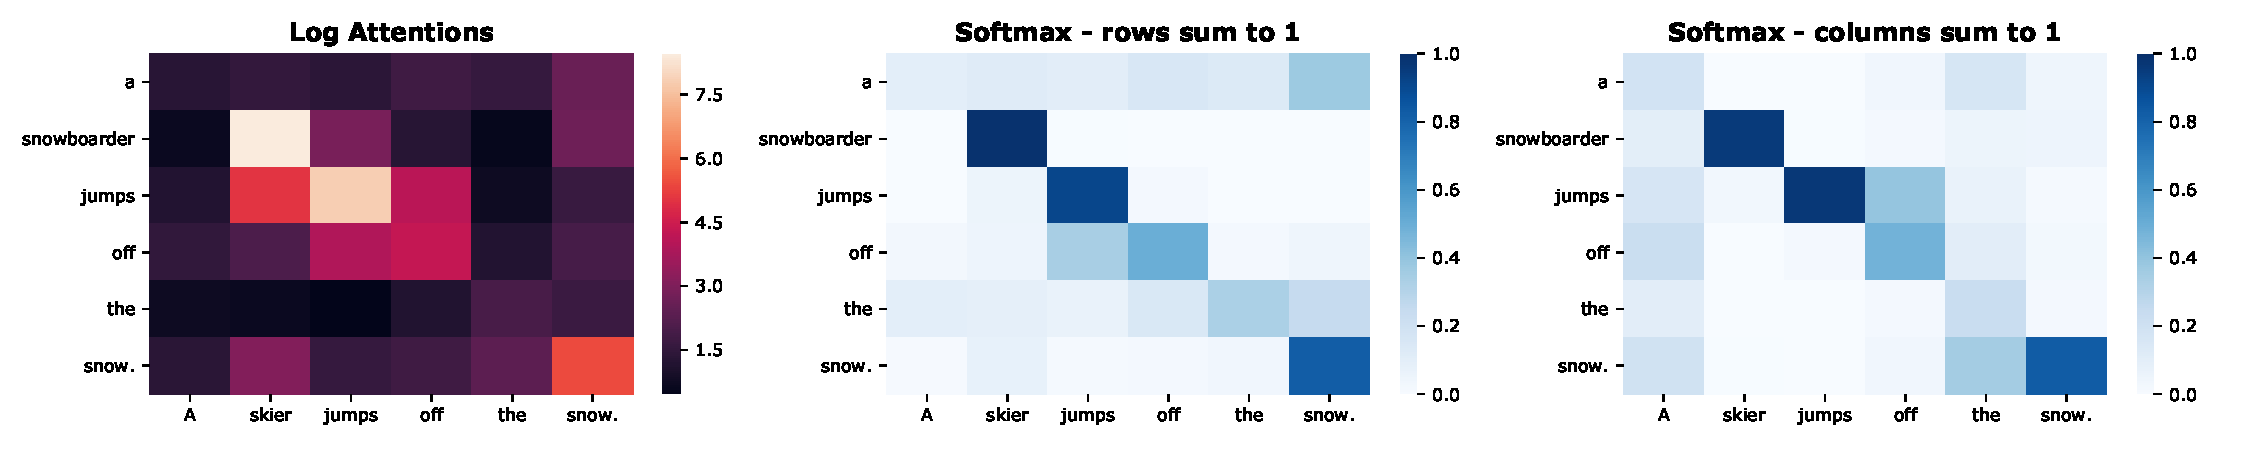
\includegraphics[width=\textwidth]{figs/ski-snow.pdf}
\caption{Attention weights for ski/snow sentences.}
\label{fig:skisnow}
\end{figure}

\begin{figure}[h]
\centering
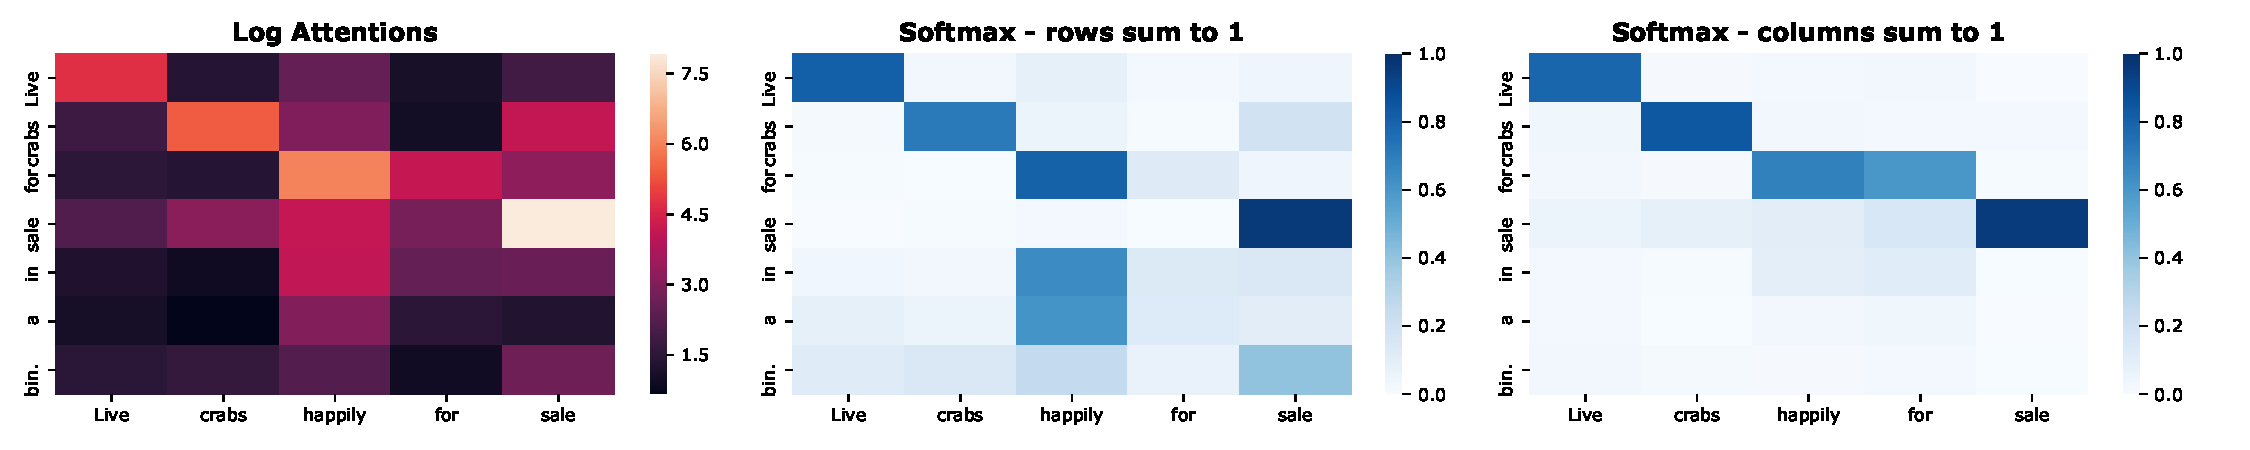
\includegraphics[width=\textwidth]{figs/crabs.pdf}
\caption{Attention weights for crabs example}
\label{fig:crabs}
\end{figure}

\begin{figure}[h]
\centering
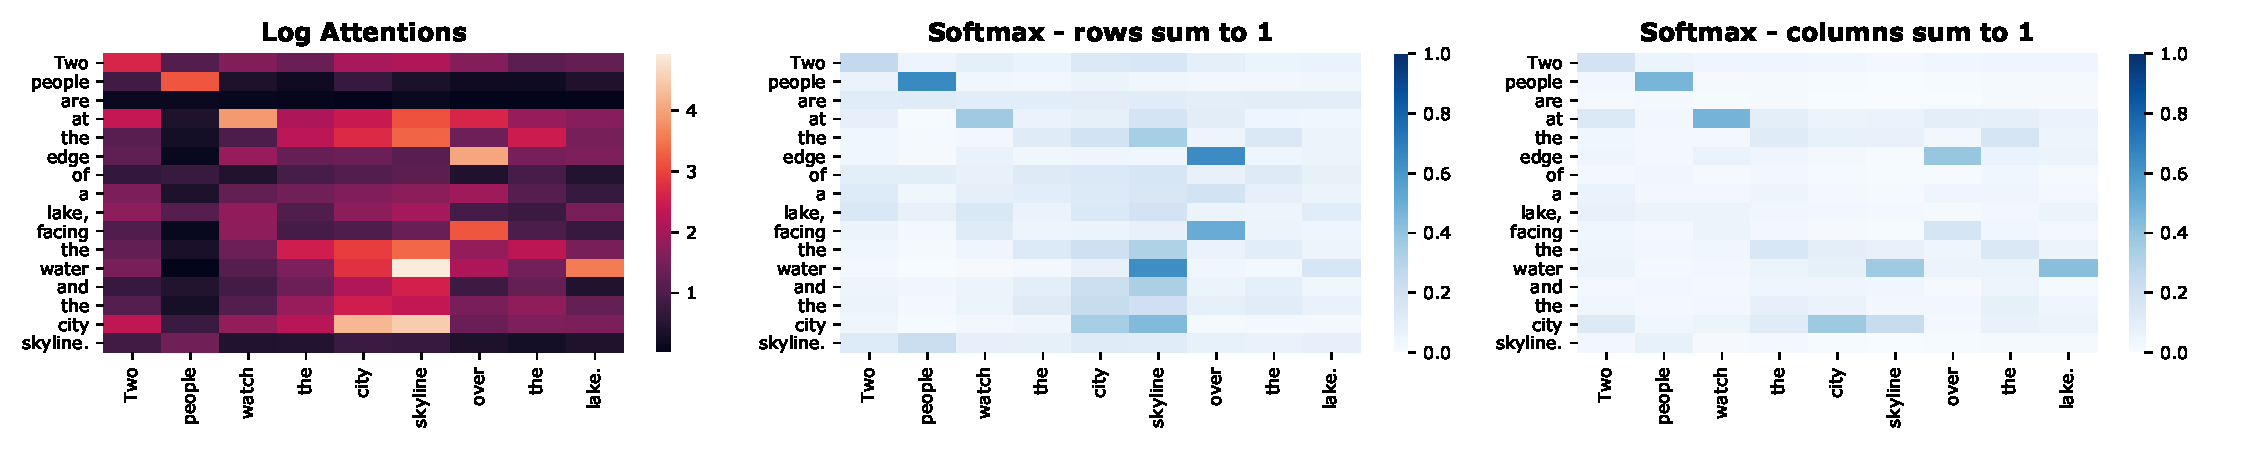
\includegraphics[width=\textwidth]{figs/skyline.pdf}
\caption{Attention weights for skyline example}
\label{fig:skyline}
\end{figure}

\bibliographystyle{apalike}
\bibliography{writeup}

\appendix
\section{Model implementations}
\lstinputlisting[caption={Decomposable Attention}]{../models/decomp_attn.py}

\lstinputlisting[caption={Exact Ensemble}]{../models/ensemble.py}

\lstinputlisting[caption={VAE Ensemble}]{../models/vae_ensemble.py}

% This is a test for merging
% QED





\end{document}
